%Preámbulo:  
\documentclass{article} %O cualquier otra clase.  
\usepackage[T1]{fontenc}  
\usepackage[utf8]{inputenc}  
\usepackage[spanish]{babel}  
\usepackage{amsmath,amssymb}
\usepackage[export]{adjustbox}
\usepackage[affil-it]{authblk}
\usepackage[center]{caption}
\usepackage{hyperref}
\hypersetup{
    colorlinks=true,
    linkcolor=black,      
    pdftitle={Nuclear Physics - Computer Lab 1},
    }
\usepackage{graphicx}
\graphicspath{ {C:/Users/luisf/OneDrive - UNIVERSIDAD ALICANTE/UA/Física/Cuarto/1º Cuatrimestre/Introducción a la modelizacion en física/Ejercicios/Bloque 1/Ejercicio 6/Imagenes} }
\author{Luis Lucas García}
\title{Resolución numérica de la ecuación de Schrödinger}
\date{\today}
\affil{Facultad de ciencias - Universidad de Alicante - Introducción a la modelización en física - Grupo L3 - Grado en física}
%Documento
\begin{document}
\maketitle
\begin{abstract}
En este documento vamos a realizar diversas simulaciones de la ecuación de Schrödinger y comentar las situaciones físicas que representan.
\end{abstract}
\tableofcontents
\pagebreak

\section{Pozo infinito}

Este es el ejercicio propuesto por el profesor, con la condición inicial que nos da.

\begin{figure}[h!]
\begin{center}
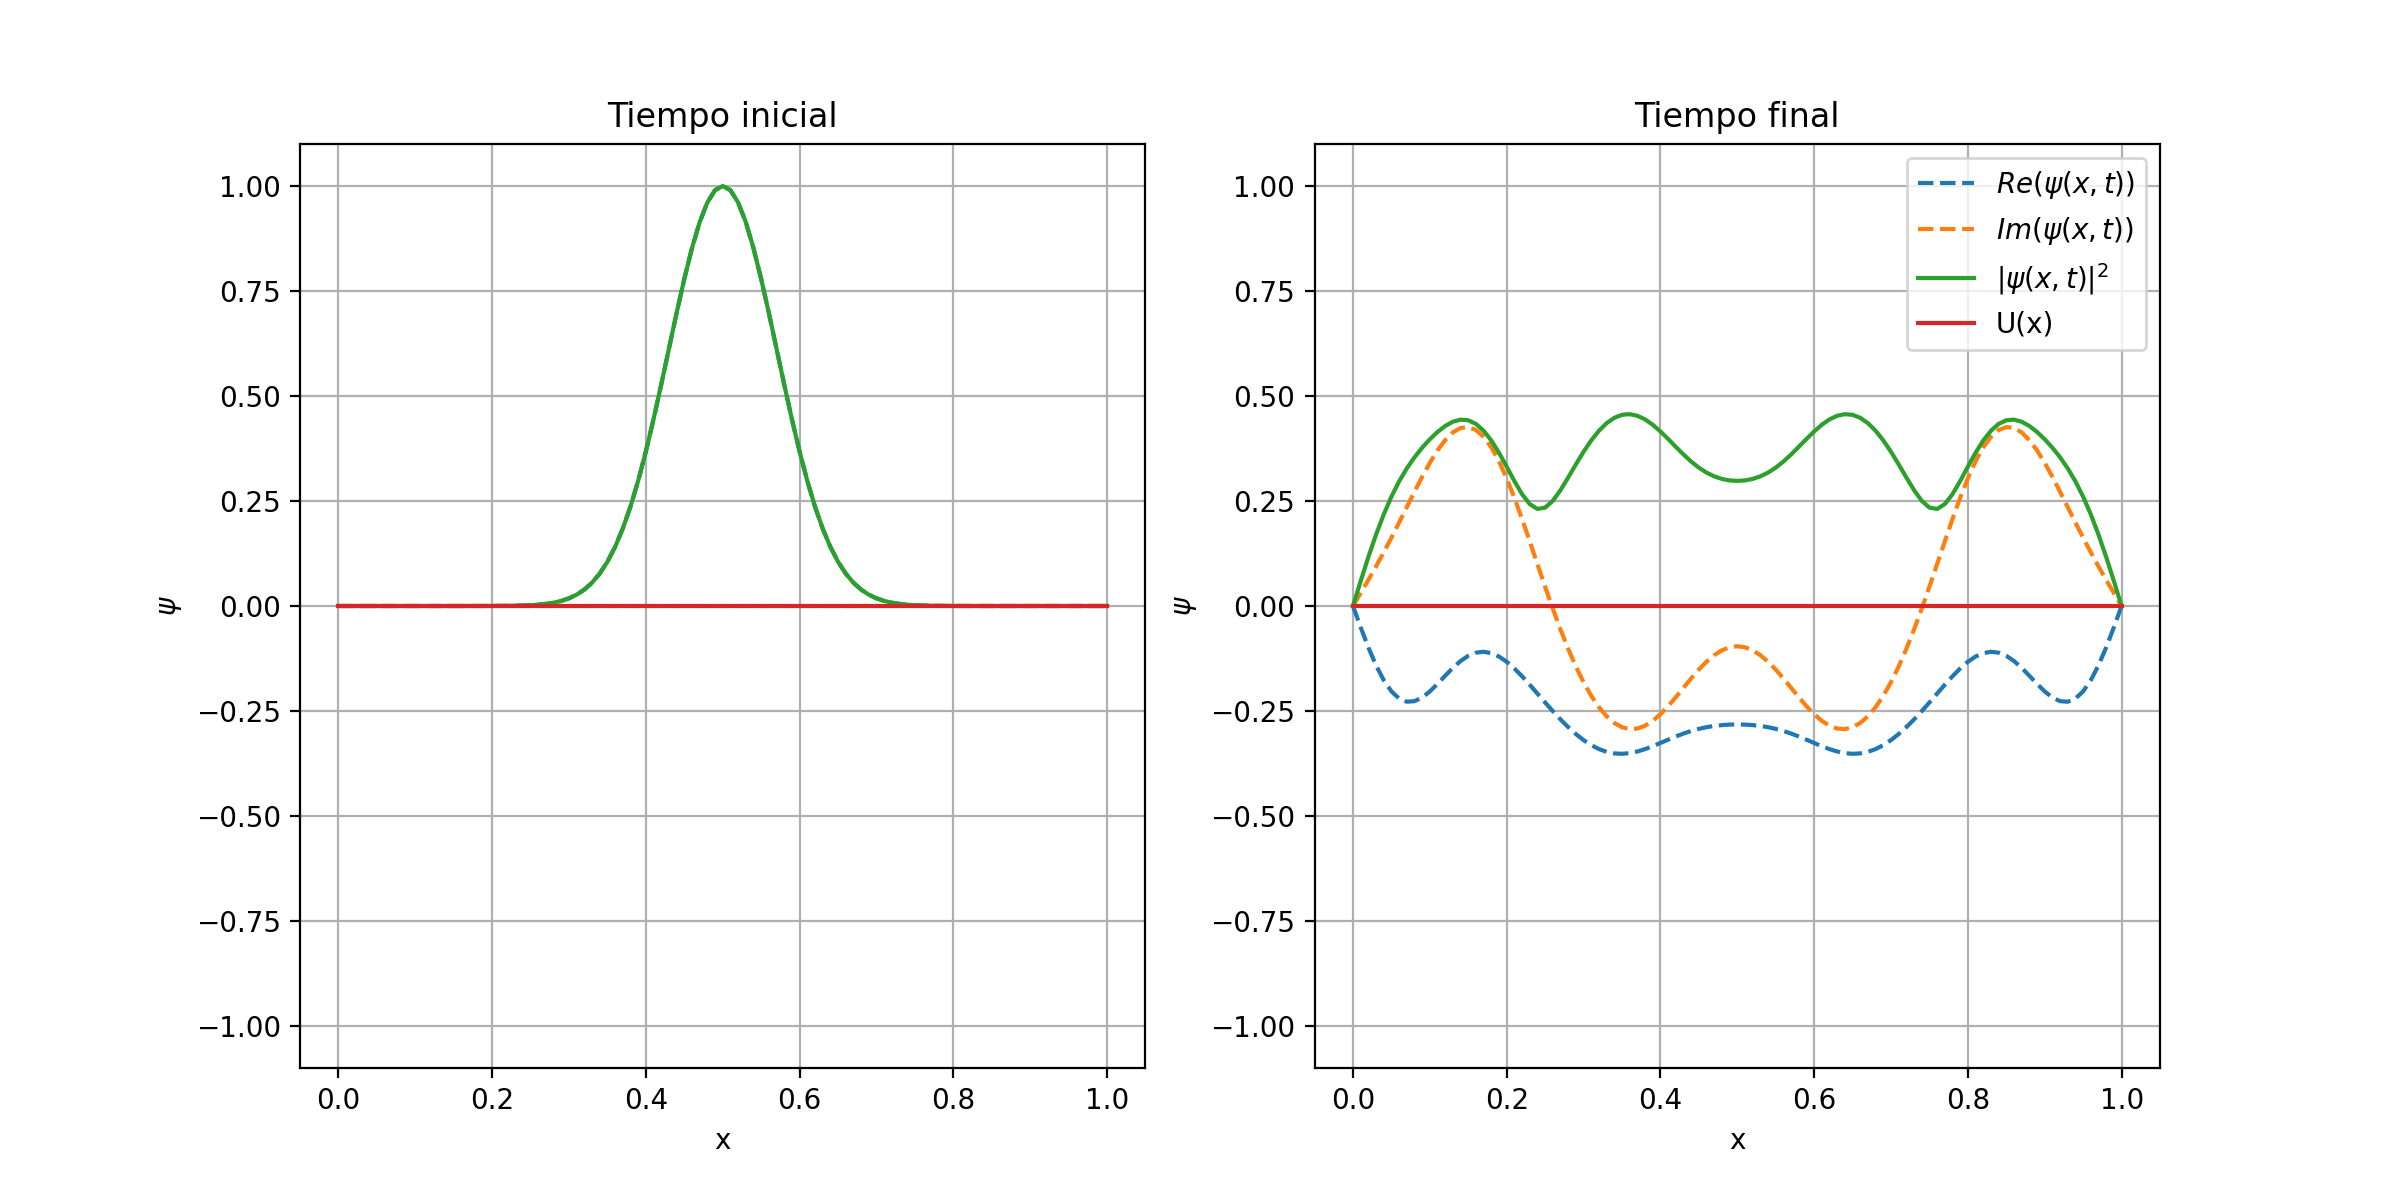
\includegraphics[max width=\linewidth]{Imagen 1 - Caso control}
\caption{Caso de control que nos da el profesor en un tiempo inicial y final}
\end{center}
\end{figure}

Si observamos la animación de dicha situación vemos que es un pozo infinito. Aquí observamos como la función de onda va oscilando entre los distintos estados estacionarios, viéndose esta oscilación, ya que el estado inicial se podría escribir como combinación lineal de los distintos estados estacionarios.

\section{Oscilador armónico}

Aquí hemos realizado la representación del primer estado excitado  de un oscilador, como es un estado estacionario se puede observar que la probabilidad de encontrar la partícula en una posición específica no cambia con el tiempo, pero las componentes real e imaginaria sí que lo hacen.

\begin{figure}[h!]
\begin{center}
\includegraphics[max width =\linewidth]{Imagen 2 - Oscilador armónico}
\caption{Representación del primer estado excitado del oscilador armónico y sus componentes. Vemos que no cambia la probabilidad con el tiempo.}
\end{center}
\end{figure}

\section{Paquete de ondas y tunelación}

Para esta sección hemos dotado a la función de onda de una condición inicial en forma de paquete de ondas. Si observamos su comportamiento, veremos que al chocar con la barrera hay parte de la probabilidad transmitida y otra reflejada, es algo similar al fenómeno de la tunelación cuántica. Tendríamos una parte reflejada y otra transmitida tras atravesar la barrera.

\begin{figure}[h!]
\begin{center}
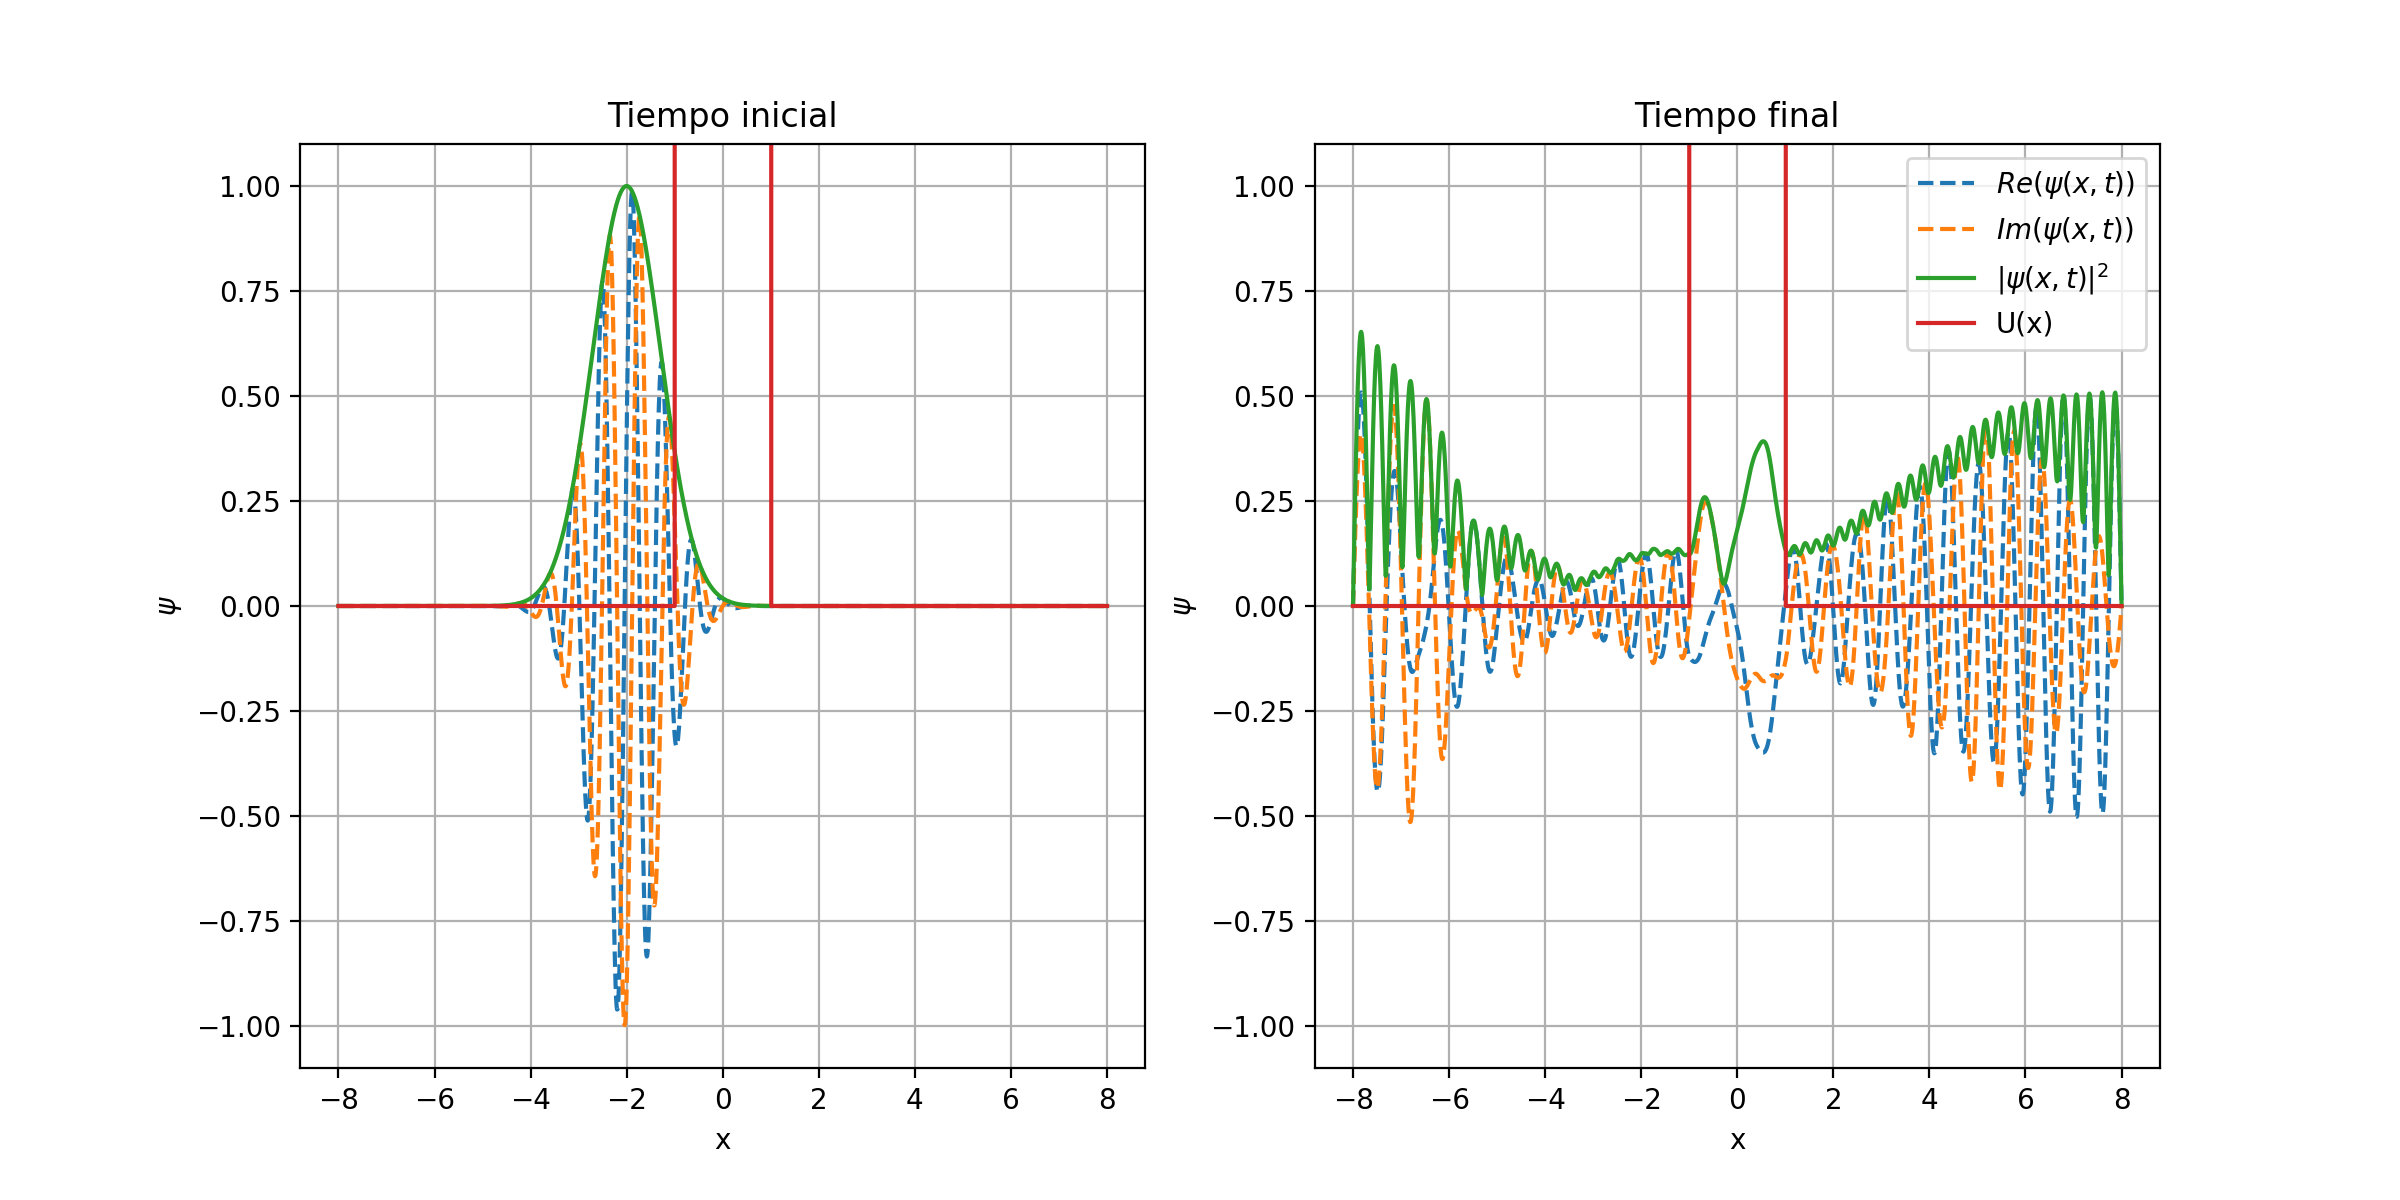
\includegraphics[max width=\linewidth]{Imagen 3 - Tunelacion}
\caption{Representación de un paquete de ondas en una barrera.}
\end{center}
\end{figure}

Siguiendo con la tunelación, también he realizado la simulación de algo que se parece a una órbita. Se puede observar como pasado un tiempo, una gran parte de la probabilidad queda confinada al pozo de potencial, lo que sería la órbita estable, pero por tunelación, parte del paquete de ondas consigue escapar y tenemos probabilidad de  encontrar la partícula fuera del pozo.

\begin{figure}[h!]
\begin{center}
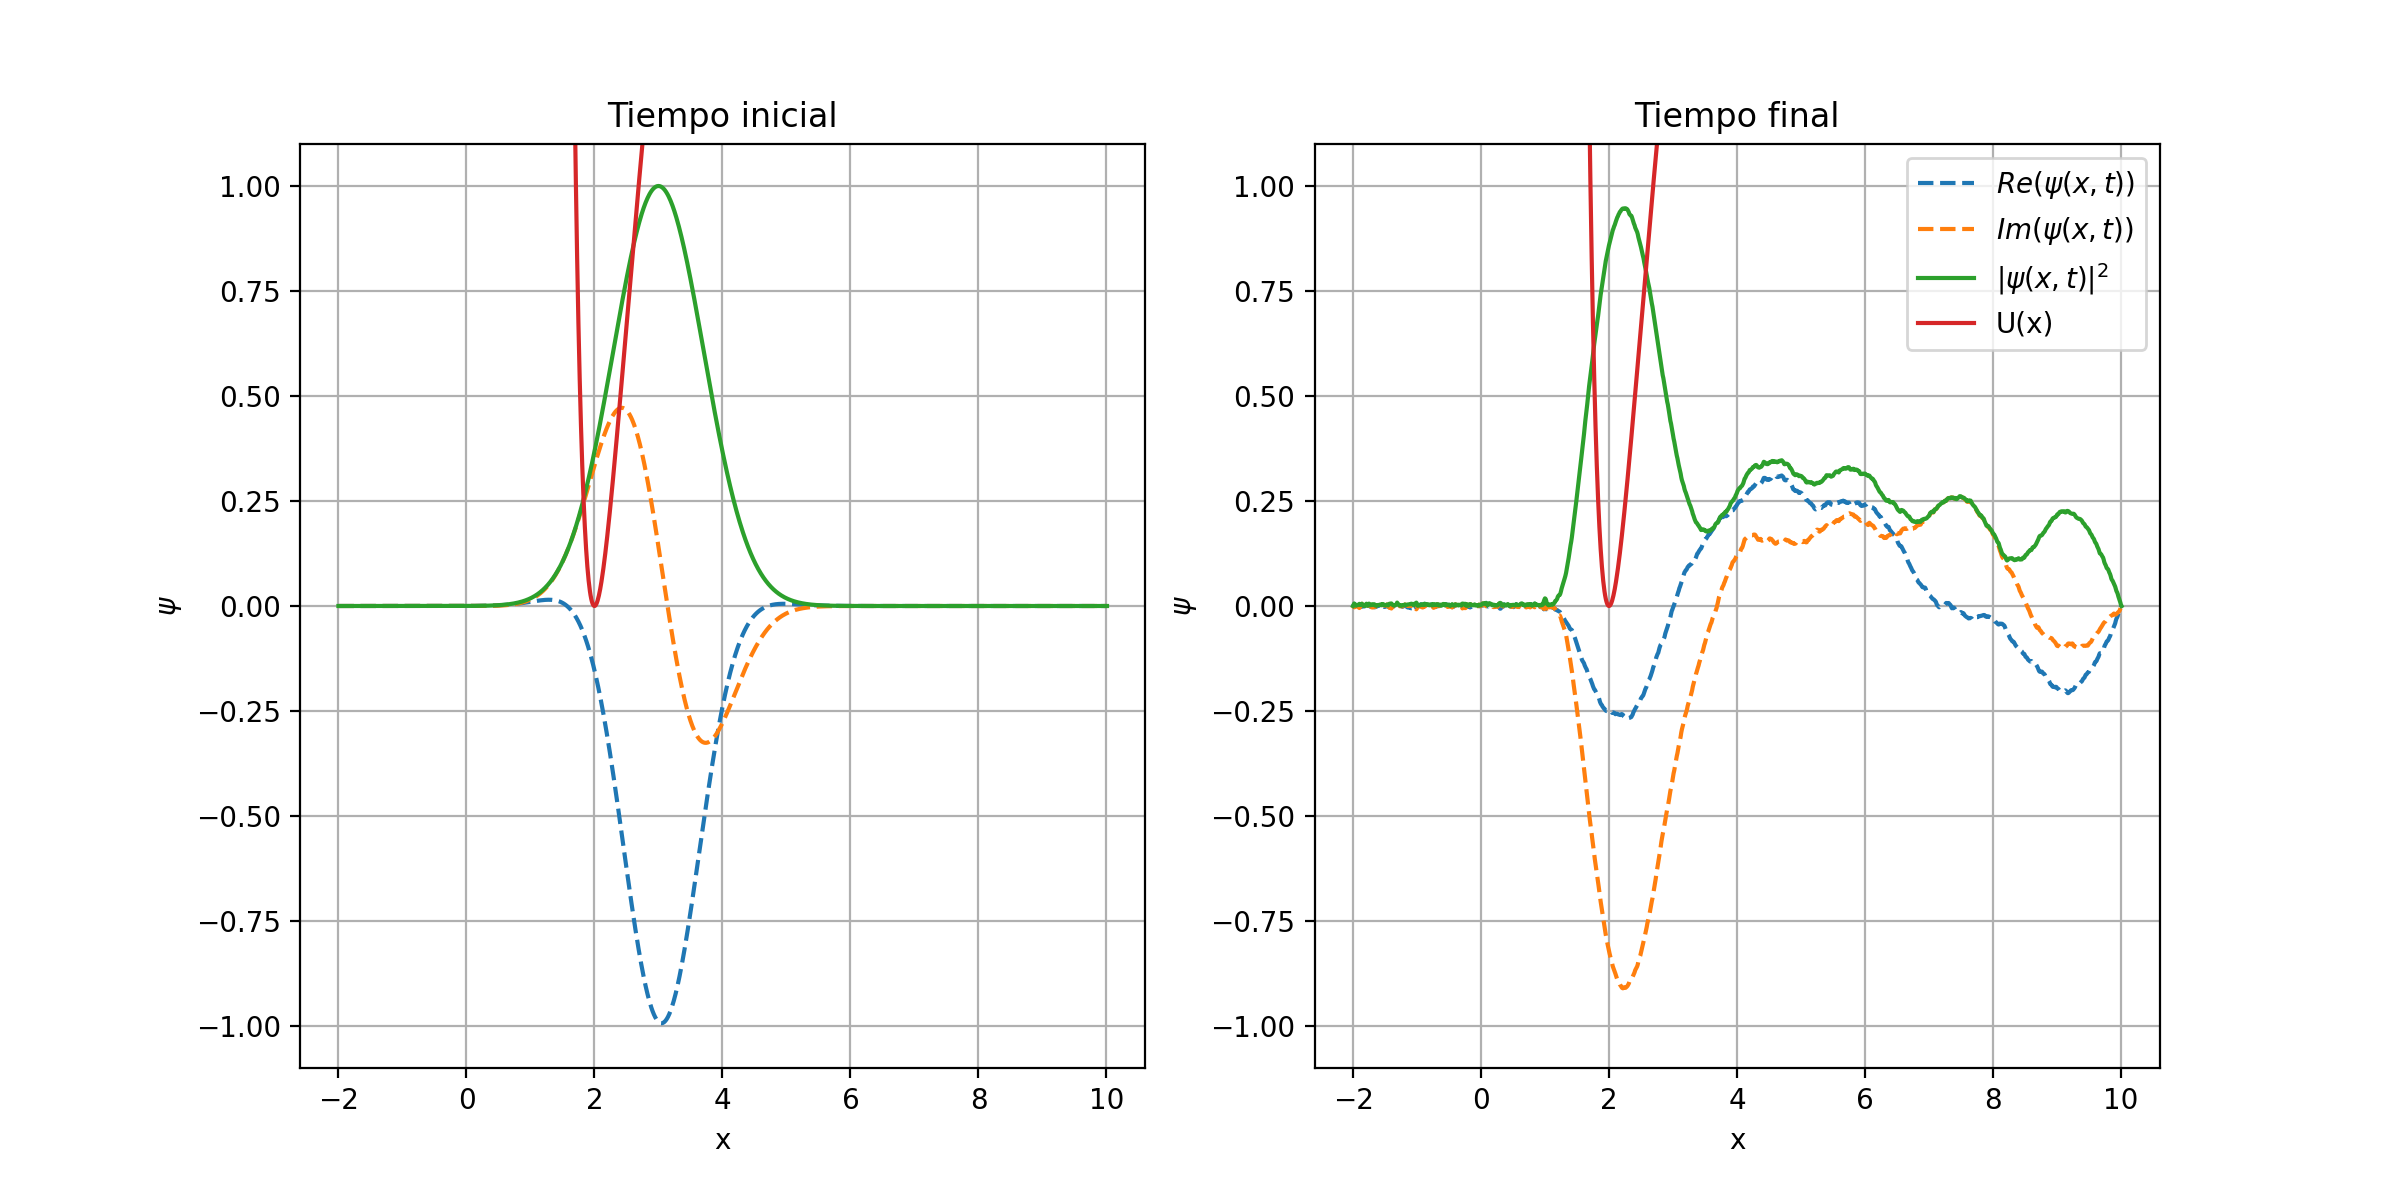
\includegraphics[max width=\linewidth]{Imagen 5 - Potencial efectivo}
\caption{Representación del caso de paquete de ondas en un potencial tipo efectivo.}
\end{center}
\end{figure}

\section{Potencial periódico}

Por último, he elegido un potencial periódico, que es algo relevante dentro de física del estado sólido. Por ejemplo, puede representar un cristal y los mínimos de potencial la posición de los iones. En este caso he intentado recrear el potencial peine de Dirac y vemos que si le dotamos de una función de onda inicial periódica, la ecuación de Schrödinger intenta mantener la periodicidad, algo que es coherente con el teorema de Bloch, pero la probabilidad se centra en el centro del pozo.

\begin{figure}[h!]
\begin{center}
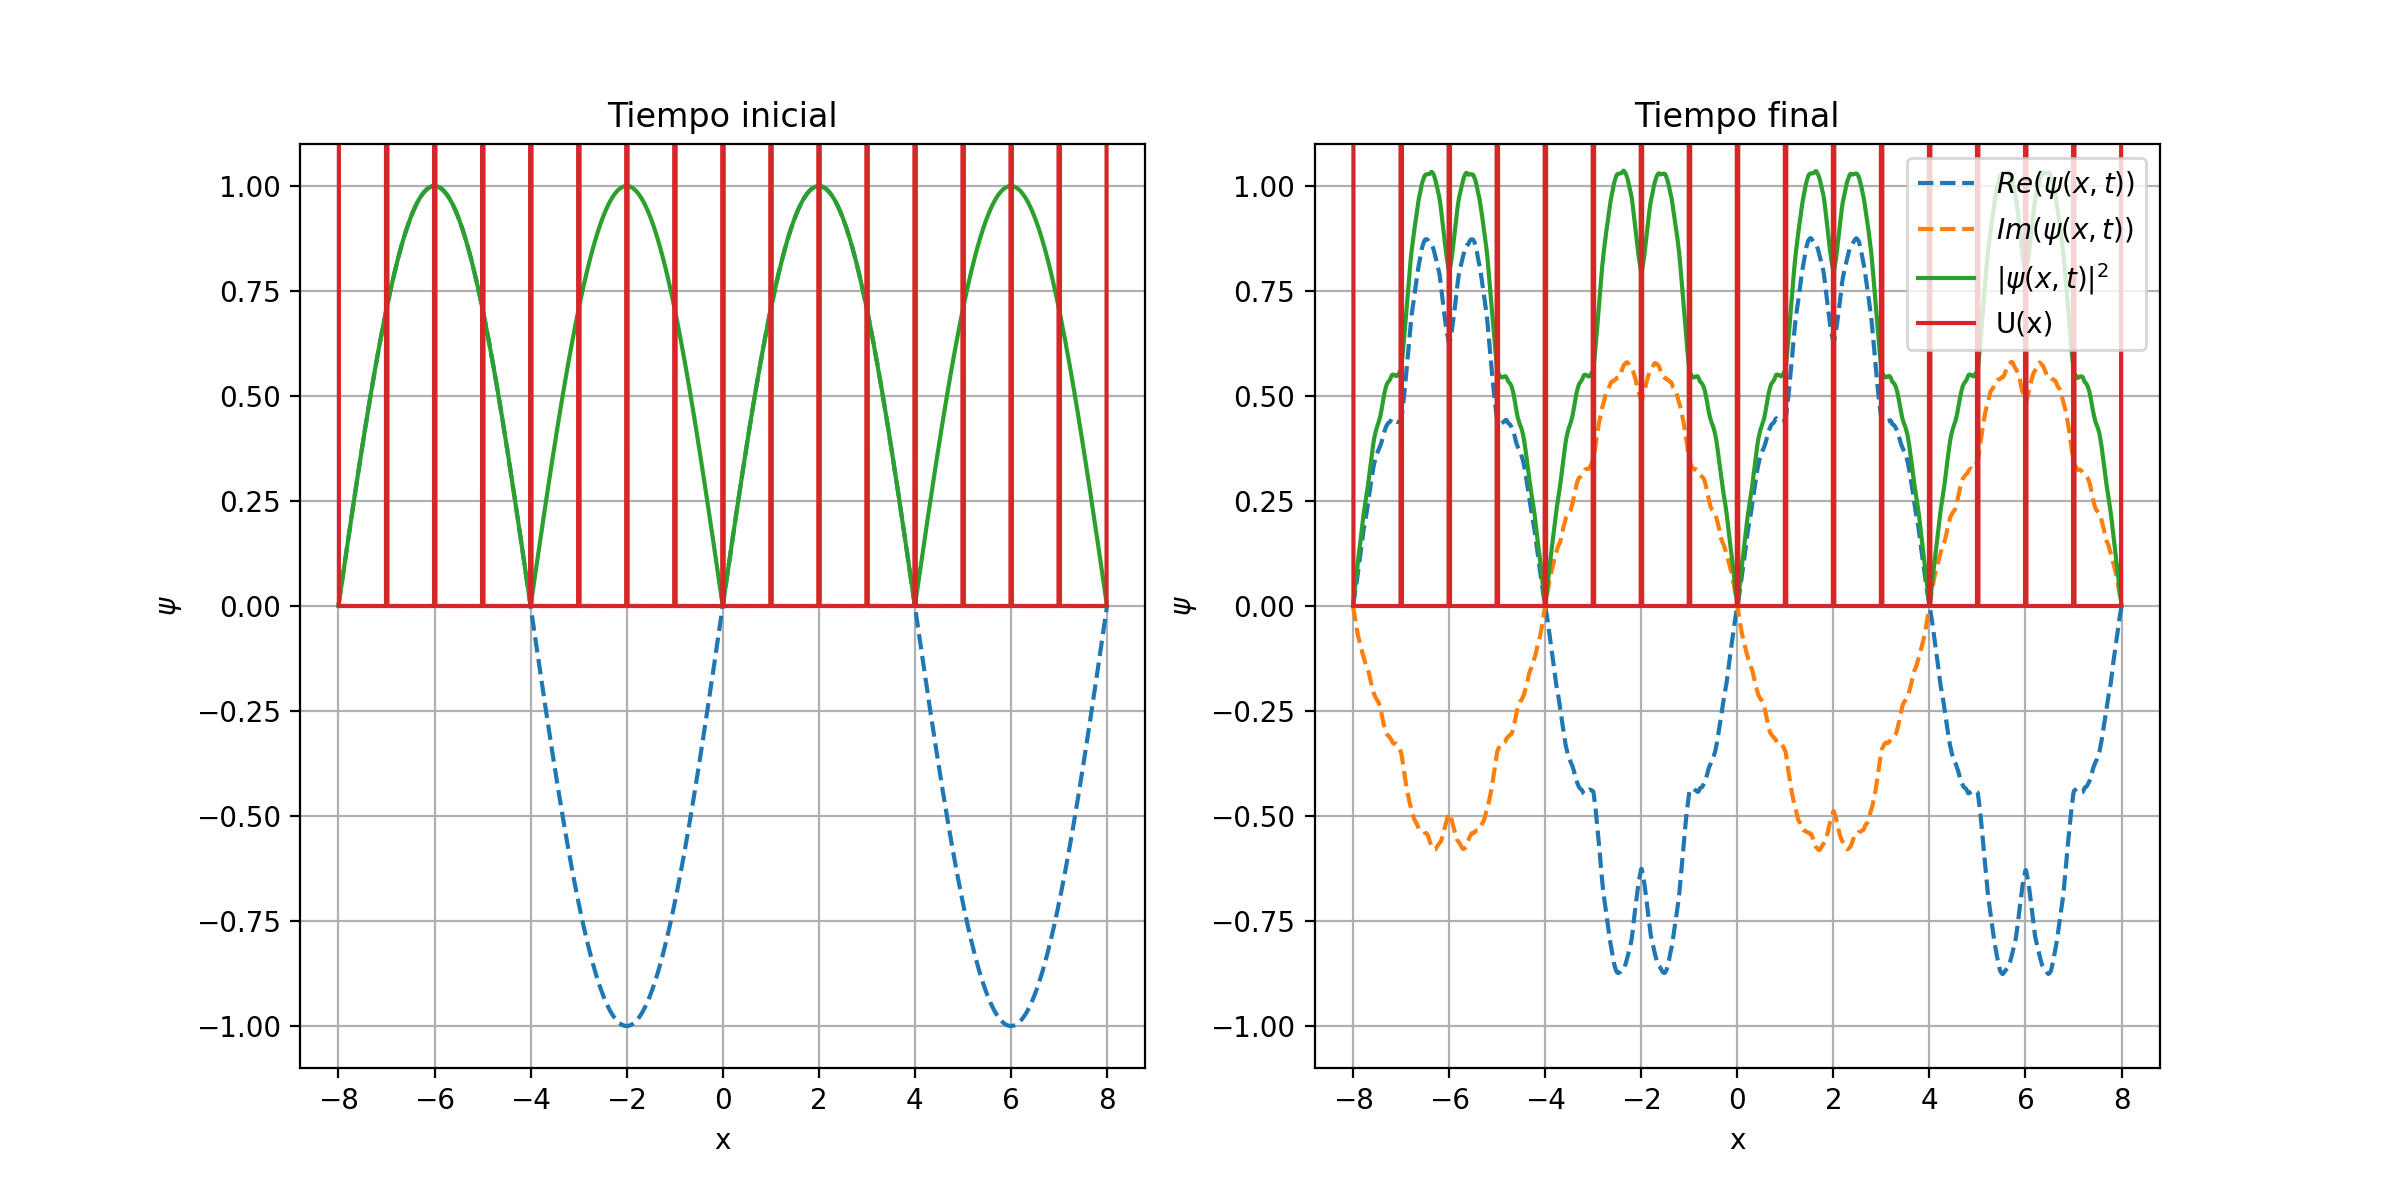
\includegraphics[max width=\linewidth]{Imagen 4 - Potencial periodico}
\caption{Representación en el potencial periódico.}
\end{center}
\end{figure}
\end{document}